\begin{figure}[t]
  \centering
  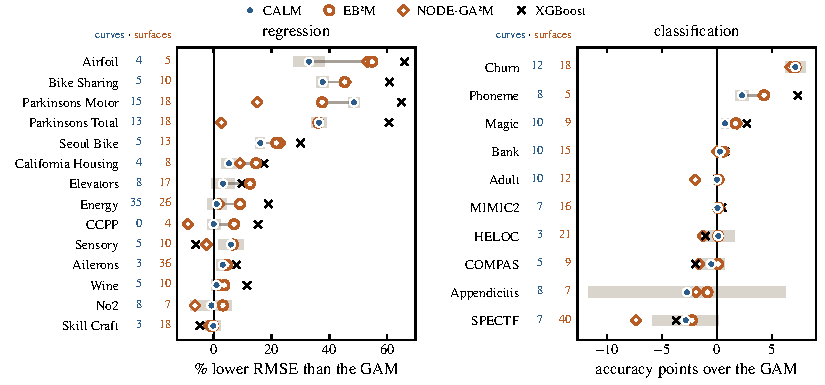
\includegraphics[width=\linewidth]{images/dumbbell}
  \caption{What each model gains over the GAM on each dataset: the black box XGBoost, the \gamms{} NODE-GA$^2$M and EB$^2$M, and \method{} (means over 5 folds, higher is better).
    The gray band behind each dot is $\pm\max(\mathrm{std}_{\text{\method{}}}, \mathrm{std}_{\text{EB}^2\text{M}})$ over the folds.
    A ring inside it is a draw, outside a win or a loss.
    \method{} ahead/level/behind:
    against the GAM, 8/6/0 in regression and 3/7/0 in classification;
    against EB$^2$M, 1/5/8 and 0/7/3 (see Tables~\ref{tab:clf-acc} and~\ref{tab:regr-rmse} for full results).
    Left of each row: the curves that \method{} adds on top of the GAM, and the pairwise surfaces that EB$^2$M fits.}
  \label{fig:dumbbell}
\end{figure}
